\section{Model for prediction}
The main step involved the prediction of any data can be organized as follows.
\begin{itemize}
    \item Data Preparation
    \item Model Creation
    \item Model Deployment
    \item Model Prediction
    \item conclusion
\end{itemize}

\subsection*{Data Preparation}
Data preparation combines many steps such as normalizing, resampling, removing tendency of the data. Normalizing is a common practice to bound the values most common may of normalizing data is to change the data range from 0 to 1. In time series, we also need to deal with the data tendency such as stationary and non-stationary. \par
\subsubsection*{Data Preparation for NonLinearRegression in PyTorch}\par
\subsubsection*{Preparation of X-data:}\par
Since year have 52-53 weeks,  I thought it's a good idea to normalize the data by the corresponding week number divided by total number of weeks in that year $X_{data} = \frac{week number}{total weeeks in that year}$. 
\subsubsection*{Preparation of Y-data:}\par
For data to normalize is much straight forward, we just normalize the data based on the maximum and minimum value. \par
\begin{equation}
    Y_{normalized} = \frac{x-x_{min}}{x_{max}-x_{min}}
    \label{eq:invarients 2}
\end{equation}
\subsubsection*{Model Selection}
There are a several forecasting models available from different open source python libraries, a few of them are \textit{scikit-learn, PyTorch,} and so on. In this work we will use \textbf{\textit{scikit-learn and PyTroch}}, the primary reason for selecting this model is flexibility and easiness of this module.\par
The \textit{PyTorch model} consists of four fully connected layers with \textit{ReLU} activation functions between them. It's designed to map input features to output features for nonlinear regression tasks, where the relationship between input and output is nonlinear. The number of hidden layers and the number of neurons in each hidden layer can be customized based on the complexity of the problem and the available data.\par
The hyperparameters can be tuned by visually assisted model performance visualizer runs on streamlit app. You can run this app in your local ZSH terminal using command \textit{poetry run streamlit run visualize \textunderscore data }.\par
The hyperparameters such as number of Epochs, Learning rate, Split between train and test data, Number of hidden neurons can be entered in the slide-box given on the right. Use can also choose to enter only specific data that can be choice by department and business ID. We can also truncate the data provided to the model by closing the start date and end date figure(\ref{fig:11.1}).\par 
\begin{figure}
    \centering
    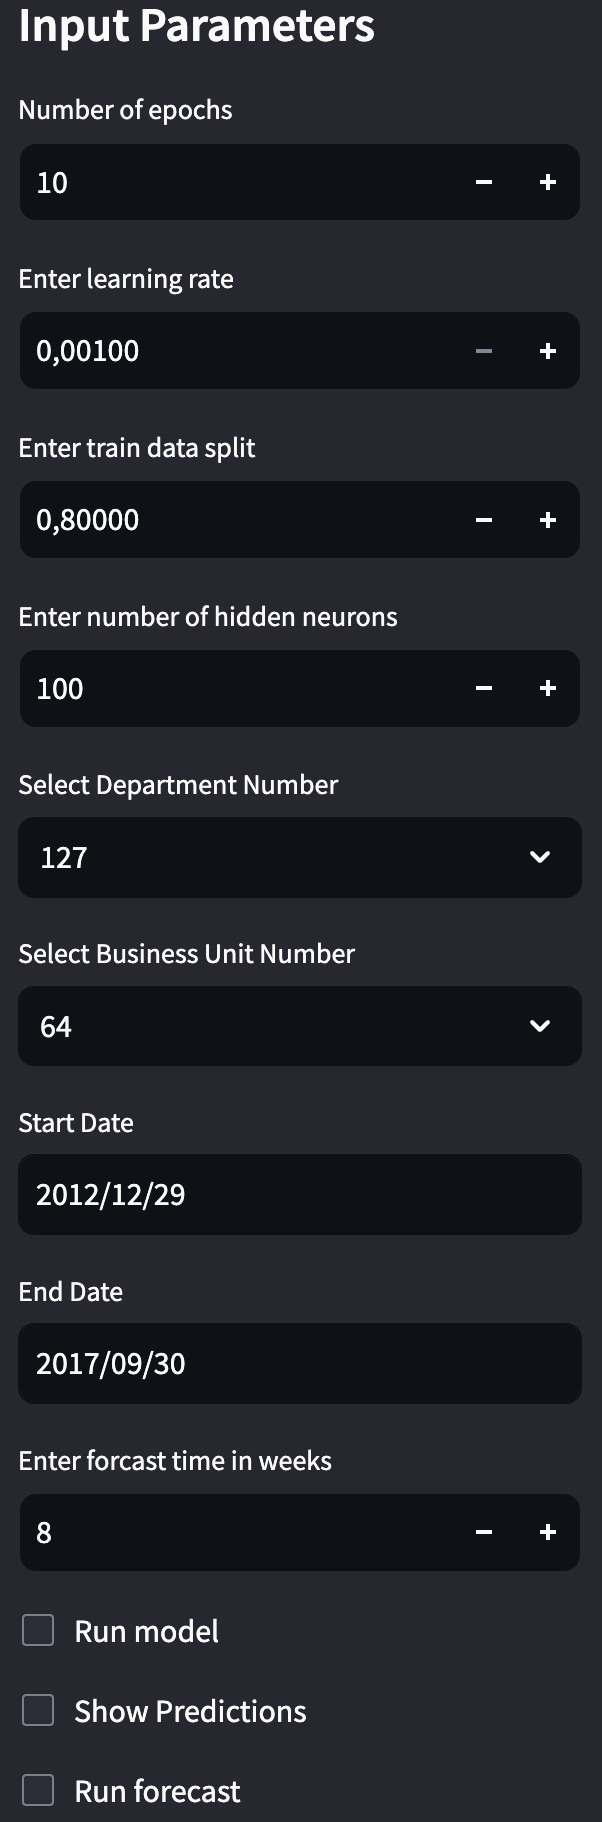
\includegraphics[width=0.4\textwidth]{figures/sidebar.png}
    \caption{Options for tuning the PyTroch model}
    \label{fig:11.1}
\end{figure}